\pagebreak
\section{Implementation}


The algorithm was implemented as discussed in section \ref{sec:algorithm} in the program called main.cpp. main.cpp has some functions for different versions of the stock market. The difference between the versions are how likely it is that two random agents will trade. For more insight see section \ref{sec:...}.\footnote{All of the programs discussed in this section can be found at \href{https://github.com/erikfsk/Project-5/tree/master/Project5}{\color{blue}{github}}}.
\\
\\
Many different simulations is needed for this report. This is why a parallelized version has been made. MPI is used since it is easy to implement. Most of the code in the parallelized version is the same as for the non-parallelized. The parallelized version should then be X times faster then the normal version with X cores. Each thread and runs the simulations for some given values for $\alpha$, $\lambda$ and $\gamma$. The values is determined by the rank of the thread and will therefor be unique to other thread's values.\footnotemark


\begin{center}
\label{tab:parallell}
\captionof{table}{The agents were given $10^7$ opportunities to do a transaction and the system was simulated 160 times. The test ran on a macbook pro 15. It has a quad core CPU. Expected difference is 4. The difference was higher, then expected. This is due to the Hyper-Threading technology in this CPU. }
\begin{tabularx}{\textwidth}{c X c X c X c X c}
    \hline 
    \hline 
       	Version && Normal && MPI && Expected difference && Actual difference\\ 
    \hline
        A   	&&      35.147  s	&&		7.361 s 	&&	4.000	&&	4.774	\\  
        D   	&&      98.112  s	&&		17.202 s	&&	4.000	&&	5.764	\\
        E   	&&      226.522 s	&&		45.608 s	&&	4.000	&&	4.966	\\
    \hline
\end{tabularx}
\end{center}


\footnotetext{\href{https://www.intel.com/content/www/us/en/architecture-and-technology/hyper-threading/hyper-threading-technology.html}{\color{blue}{Intel Hyper-Threading Technology}}}

\begin{center}
\label{tab:expected-time}
\captionof{table}{
For scaling we expect a time increased proportional to the size increase. The table shows how we expect the time to develop and how it actually it develops. There is a minor difference from expected and calculated and that comes from the fact that the program does more then just the algorithm and the fact that the algorithm has not been perfectly implemented.}
\begin{tabularx}{\textwidth}{c X c X c X c X c}
    \hline 
    \hline 
        Version && \# Simulations&& Expected time && Actual time && $T_{i}$ / $T_{10}$\\ 
    \hline
        A   	&& 10  &&      x		&&		2.252 s 	&&	1.000	\\  
        A   	&& 160 &&      16x		&&		35.147 s	&&	15.60	\\
        D   	&& 10  &&      x		&&		6.229 s 	&&	1.000	\\  
        D   	&& 160 &&      16x		&&		98.112 s	&&	15.75	\\
        E   	&& 10  &&      x		&&		12.876 s 	&&	1.000	\\  
        E   	&& 160 &&      16x		&&		226.522 s	&&	17.59	\\
    \hline
\end{tabularx}
\end{center}



\begin{figure}[H]
    \centering
    \begin{subfigure}{0.19\textwidth}
        \centering
        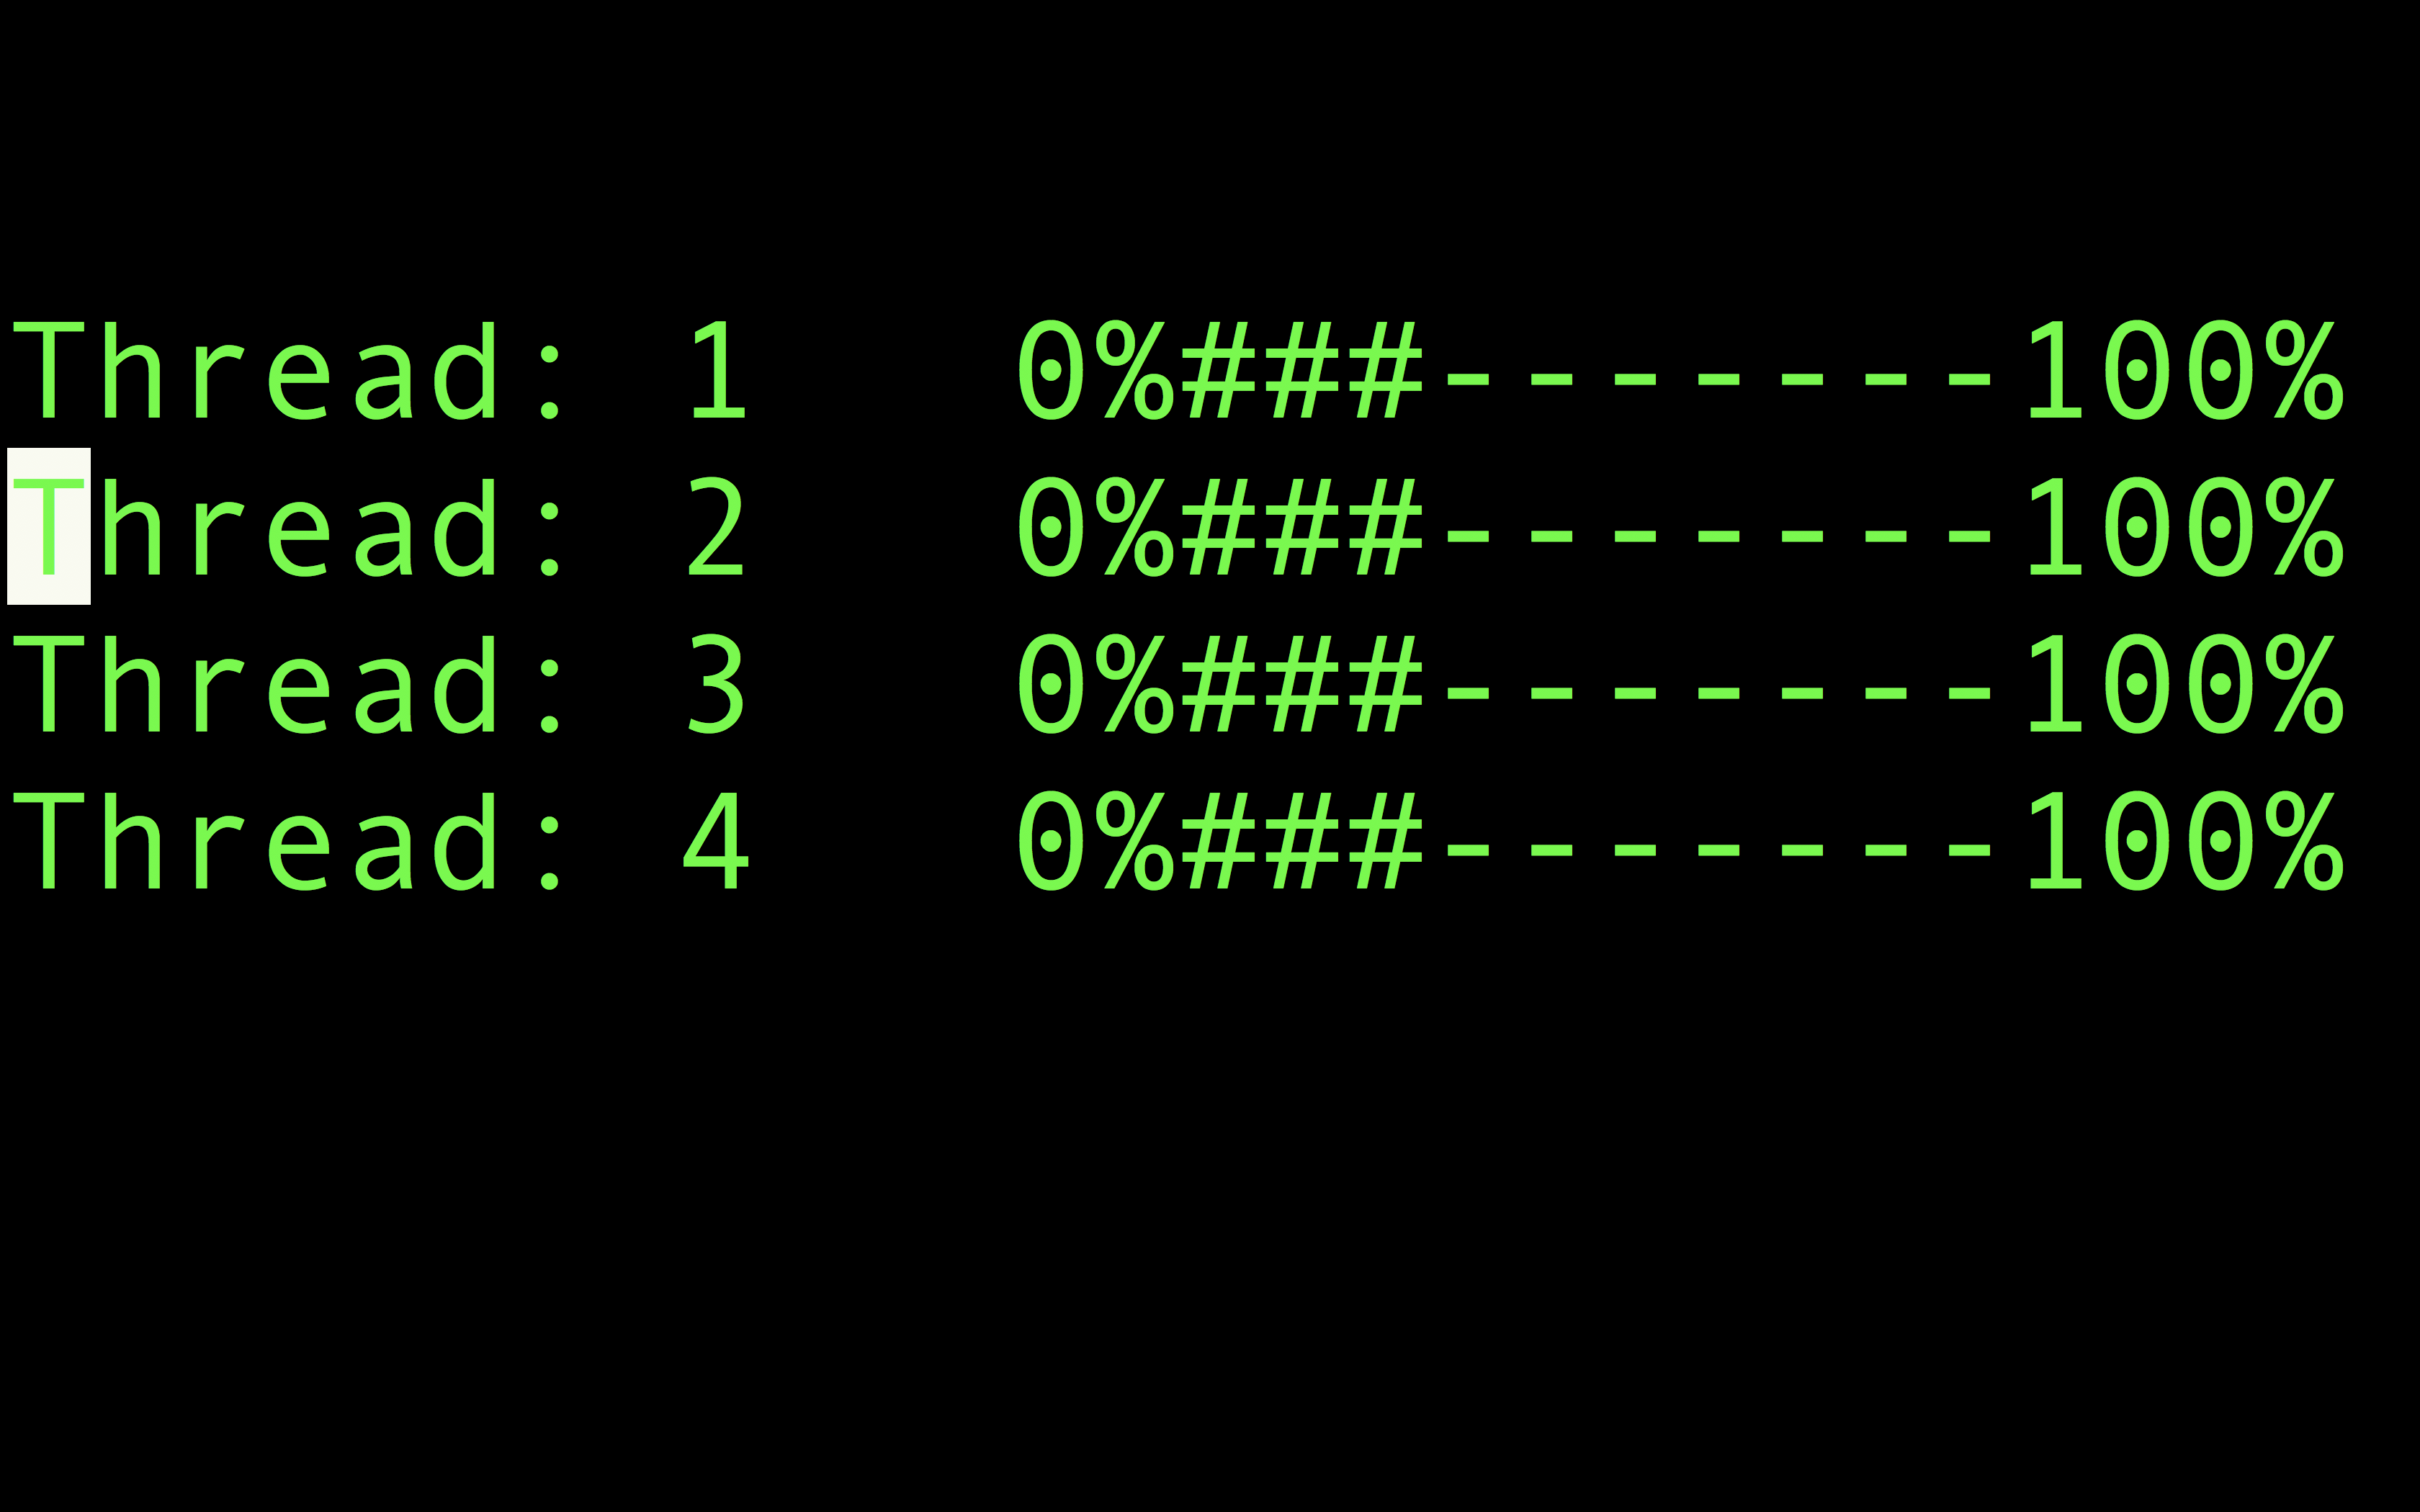
\includegraphics[width=1.11\linewidth]{method/bilder/2}
    \end{subfigure}
    ~ 
    \begin{subfigure}{0.19\textwidth}
        \centering
        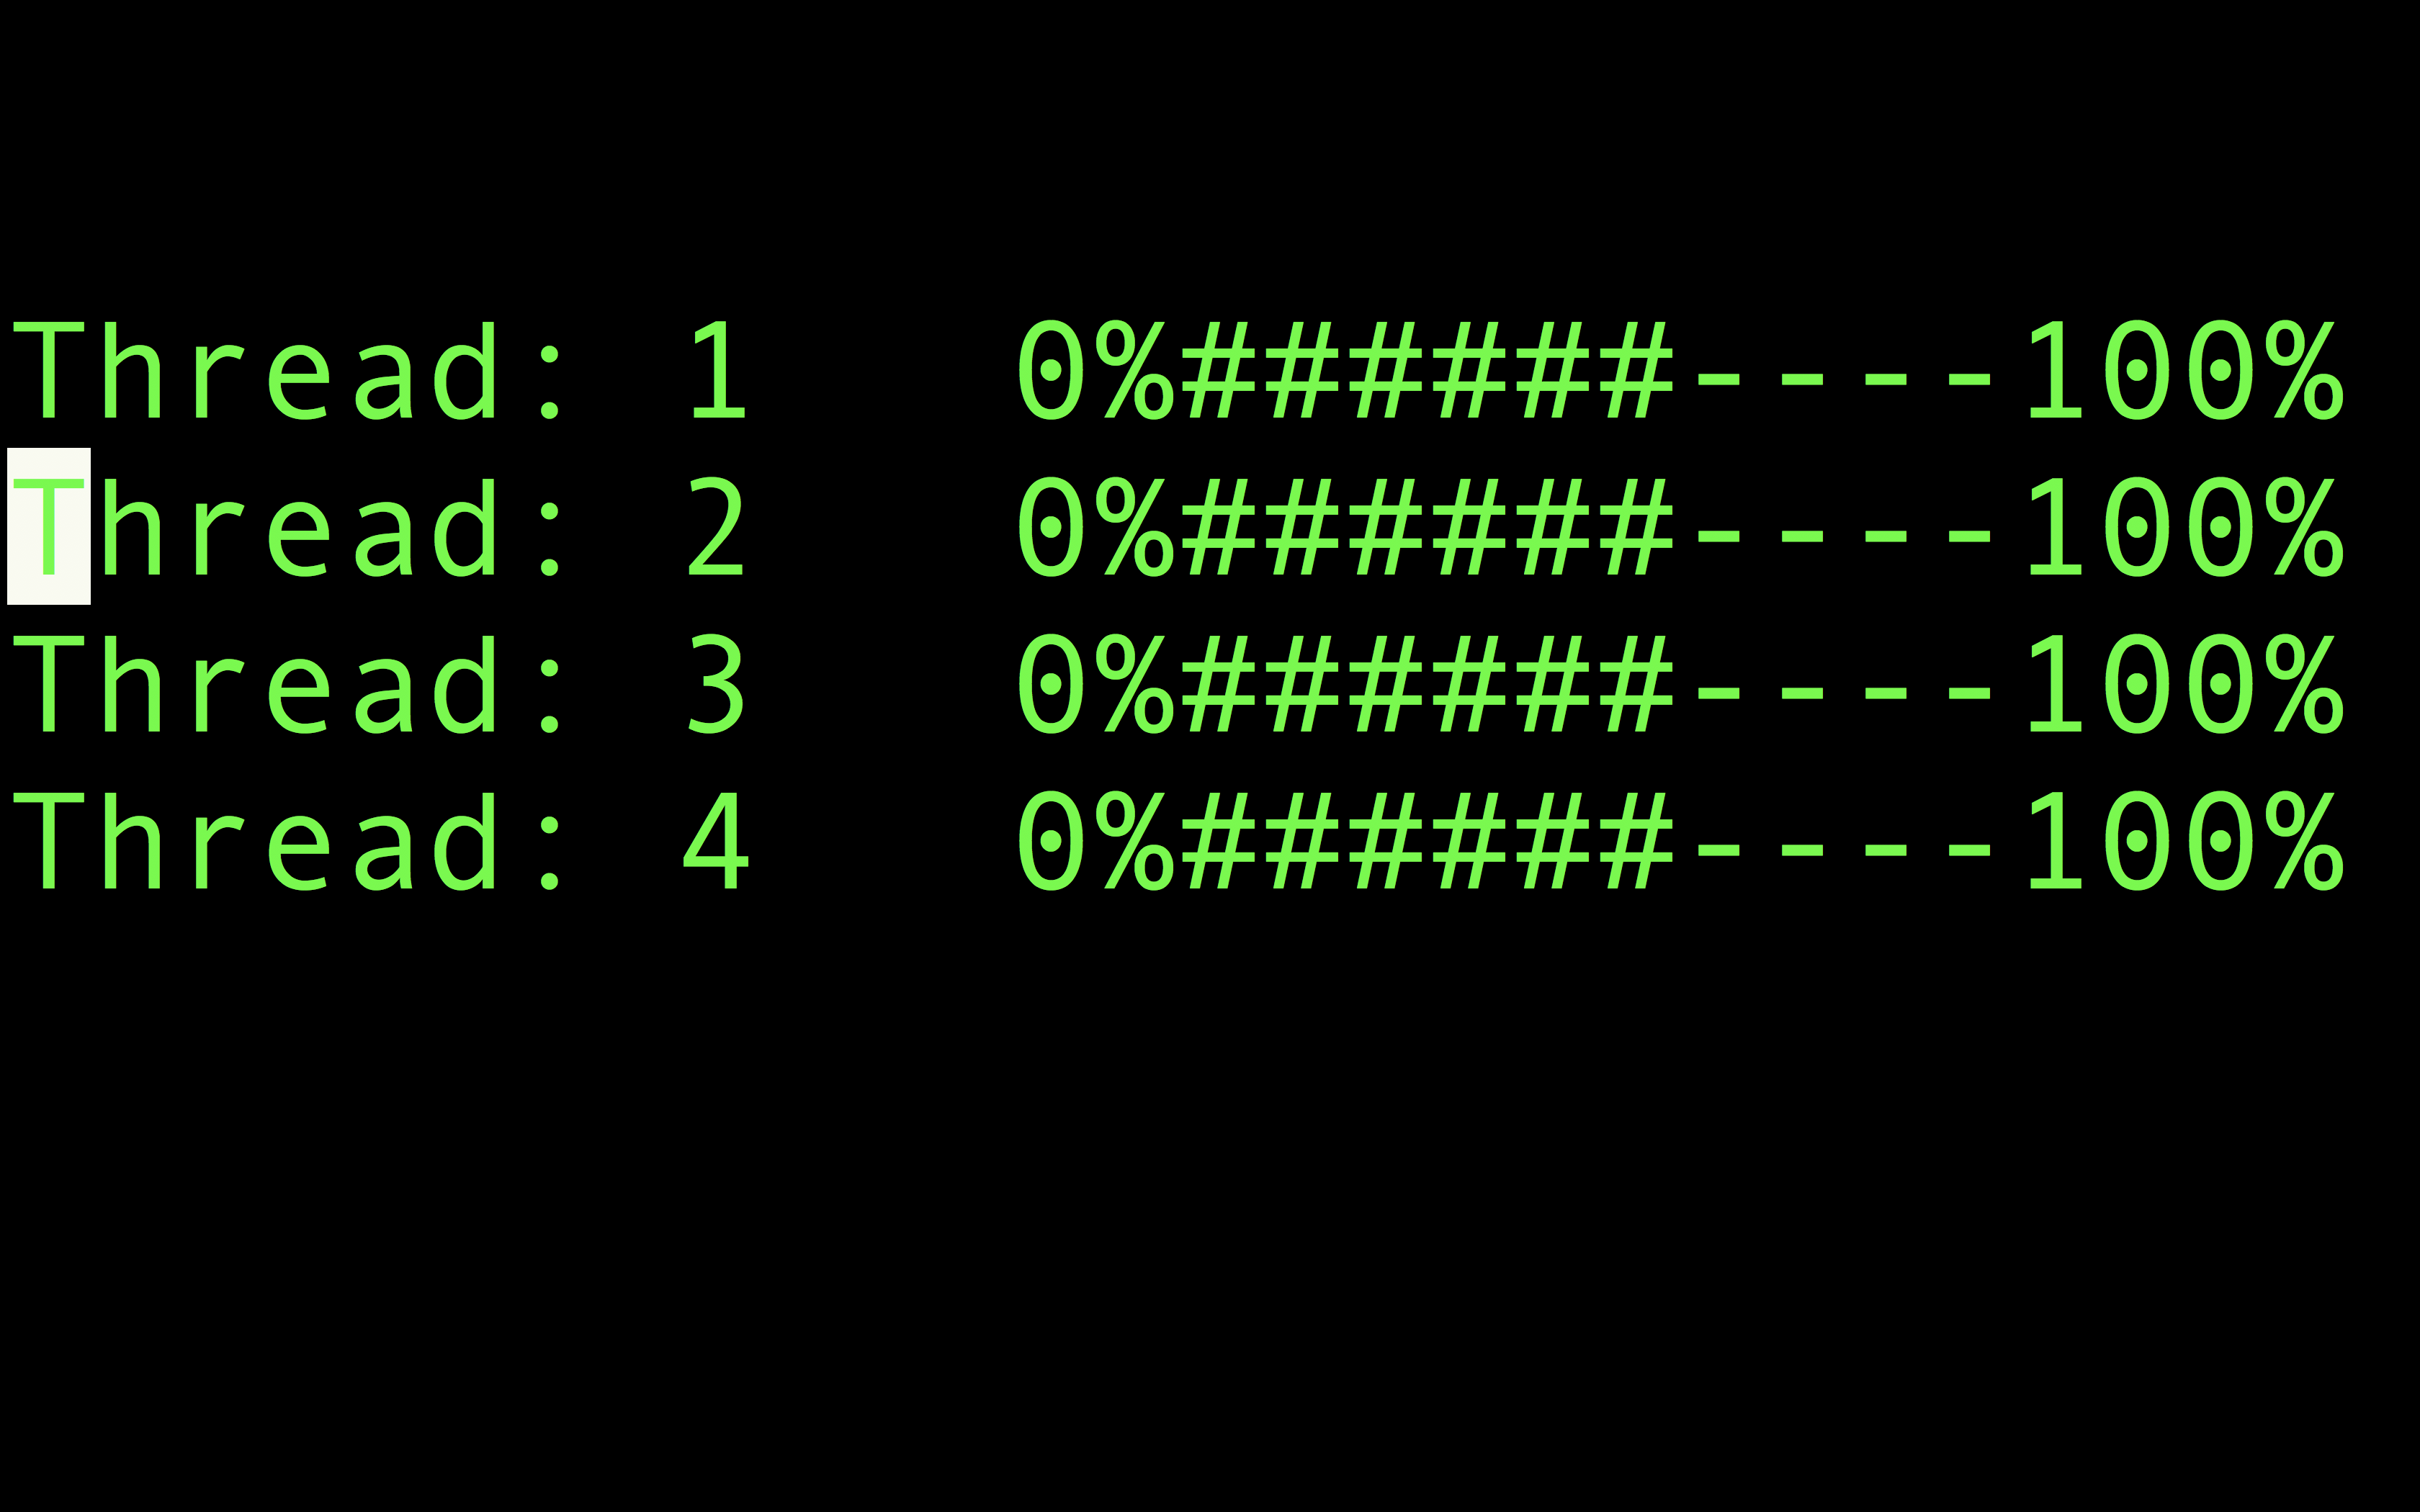
\includegraphics[width=1.11\linewidth]{method/bilder/3}
    \end{subfigure}
    ~ 
    \begin{subfigure}{0.19\textwidth}
        \centering
        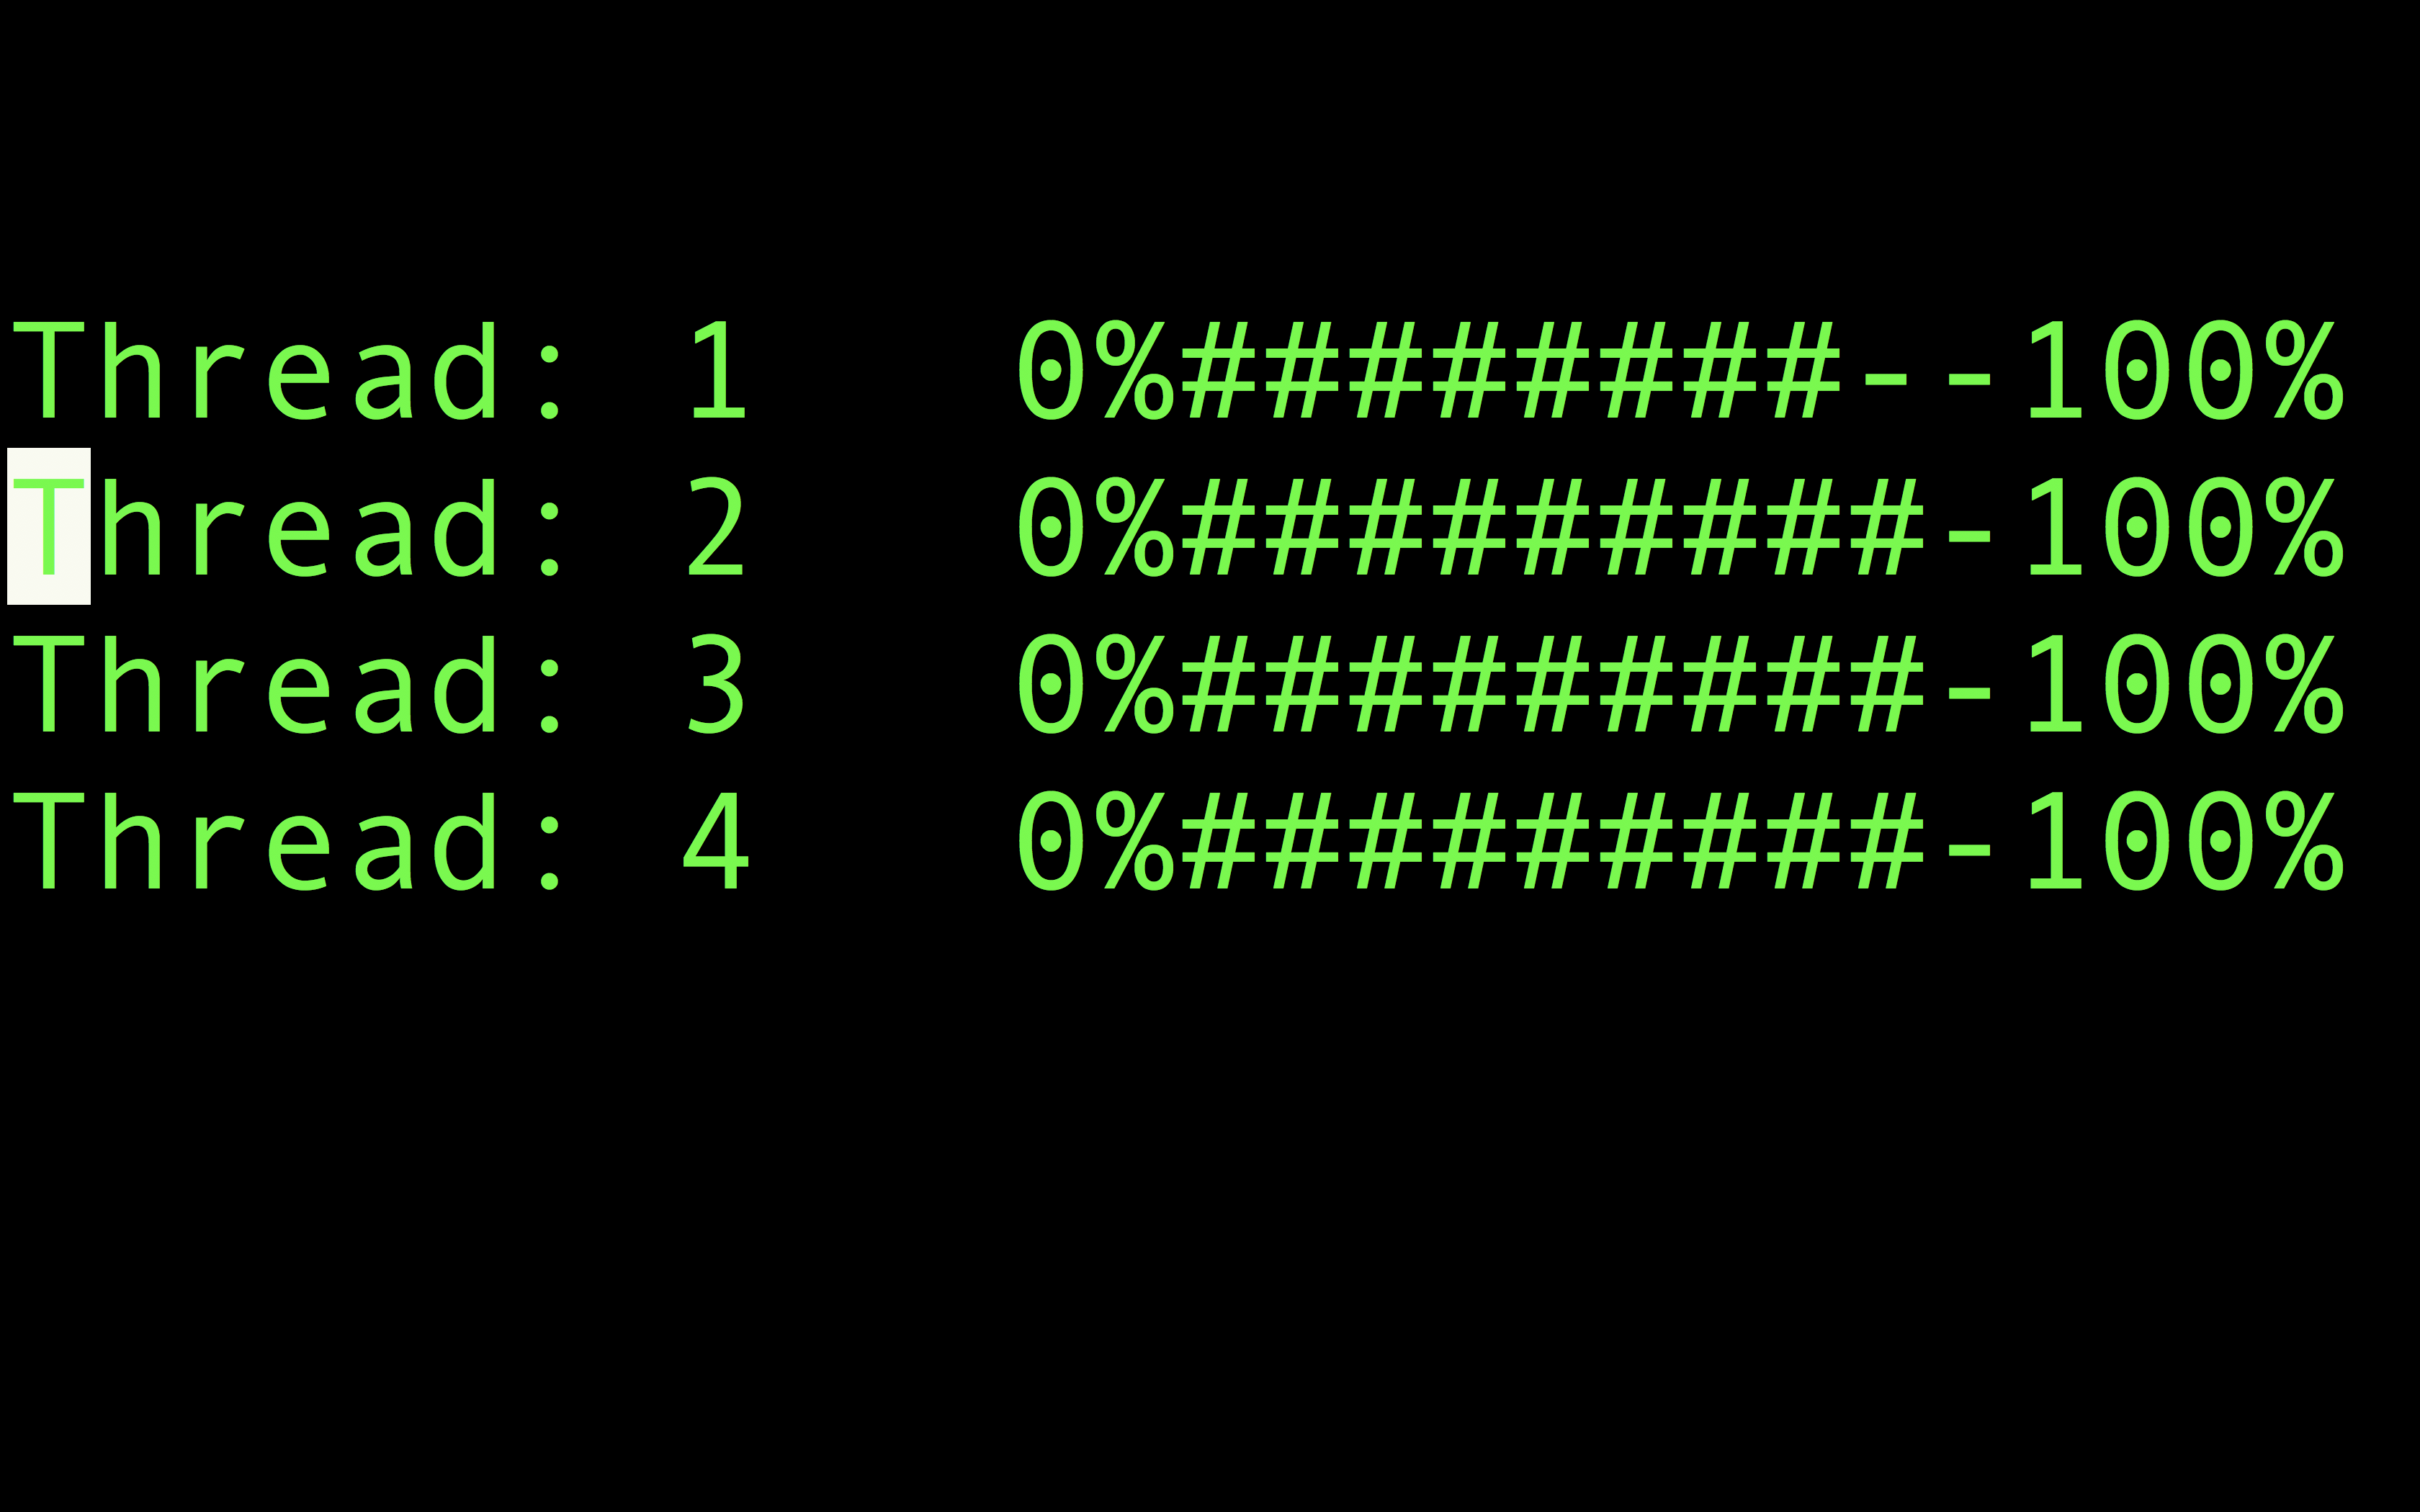
\includegraphics[width=1.11\linewidth]{method/bilder/4}
    \end{subfigure}
    ~ 
    \begin{subfigure}{0.19\textwidth}
        \centering
        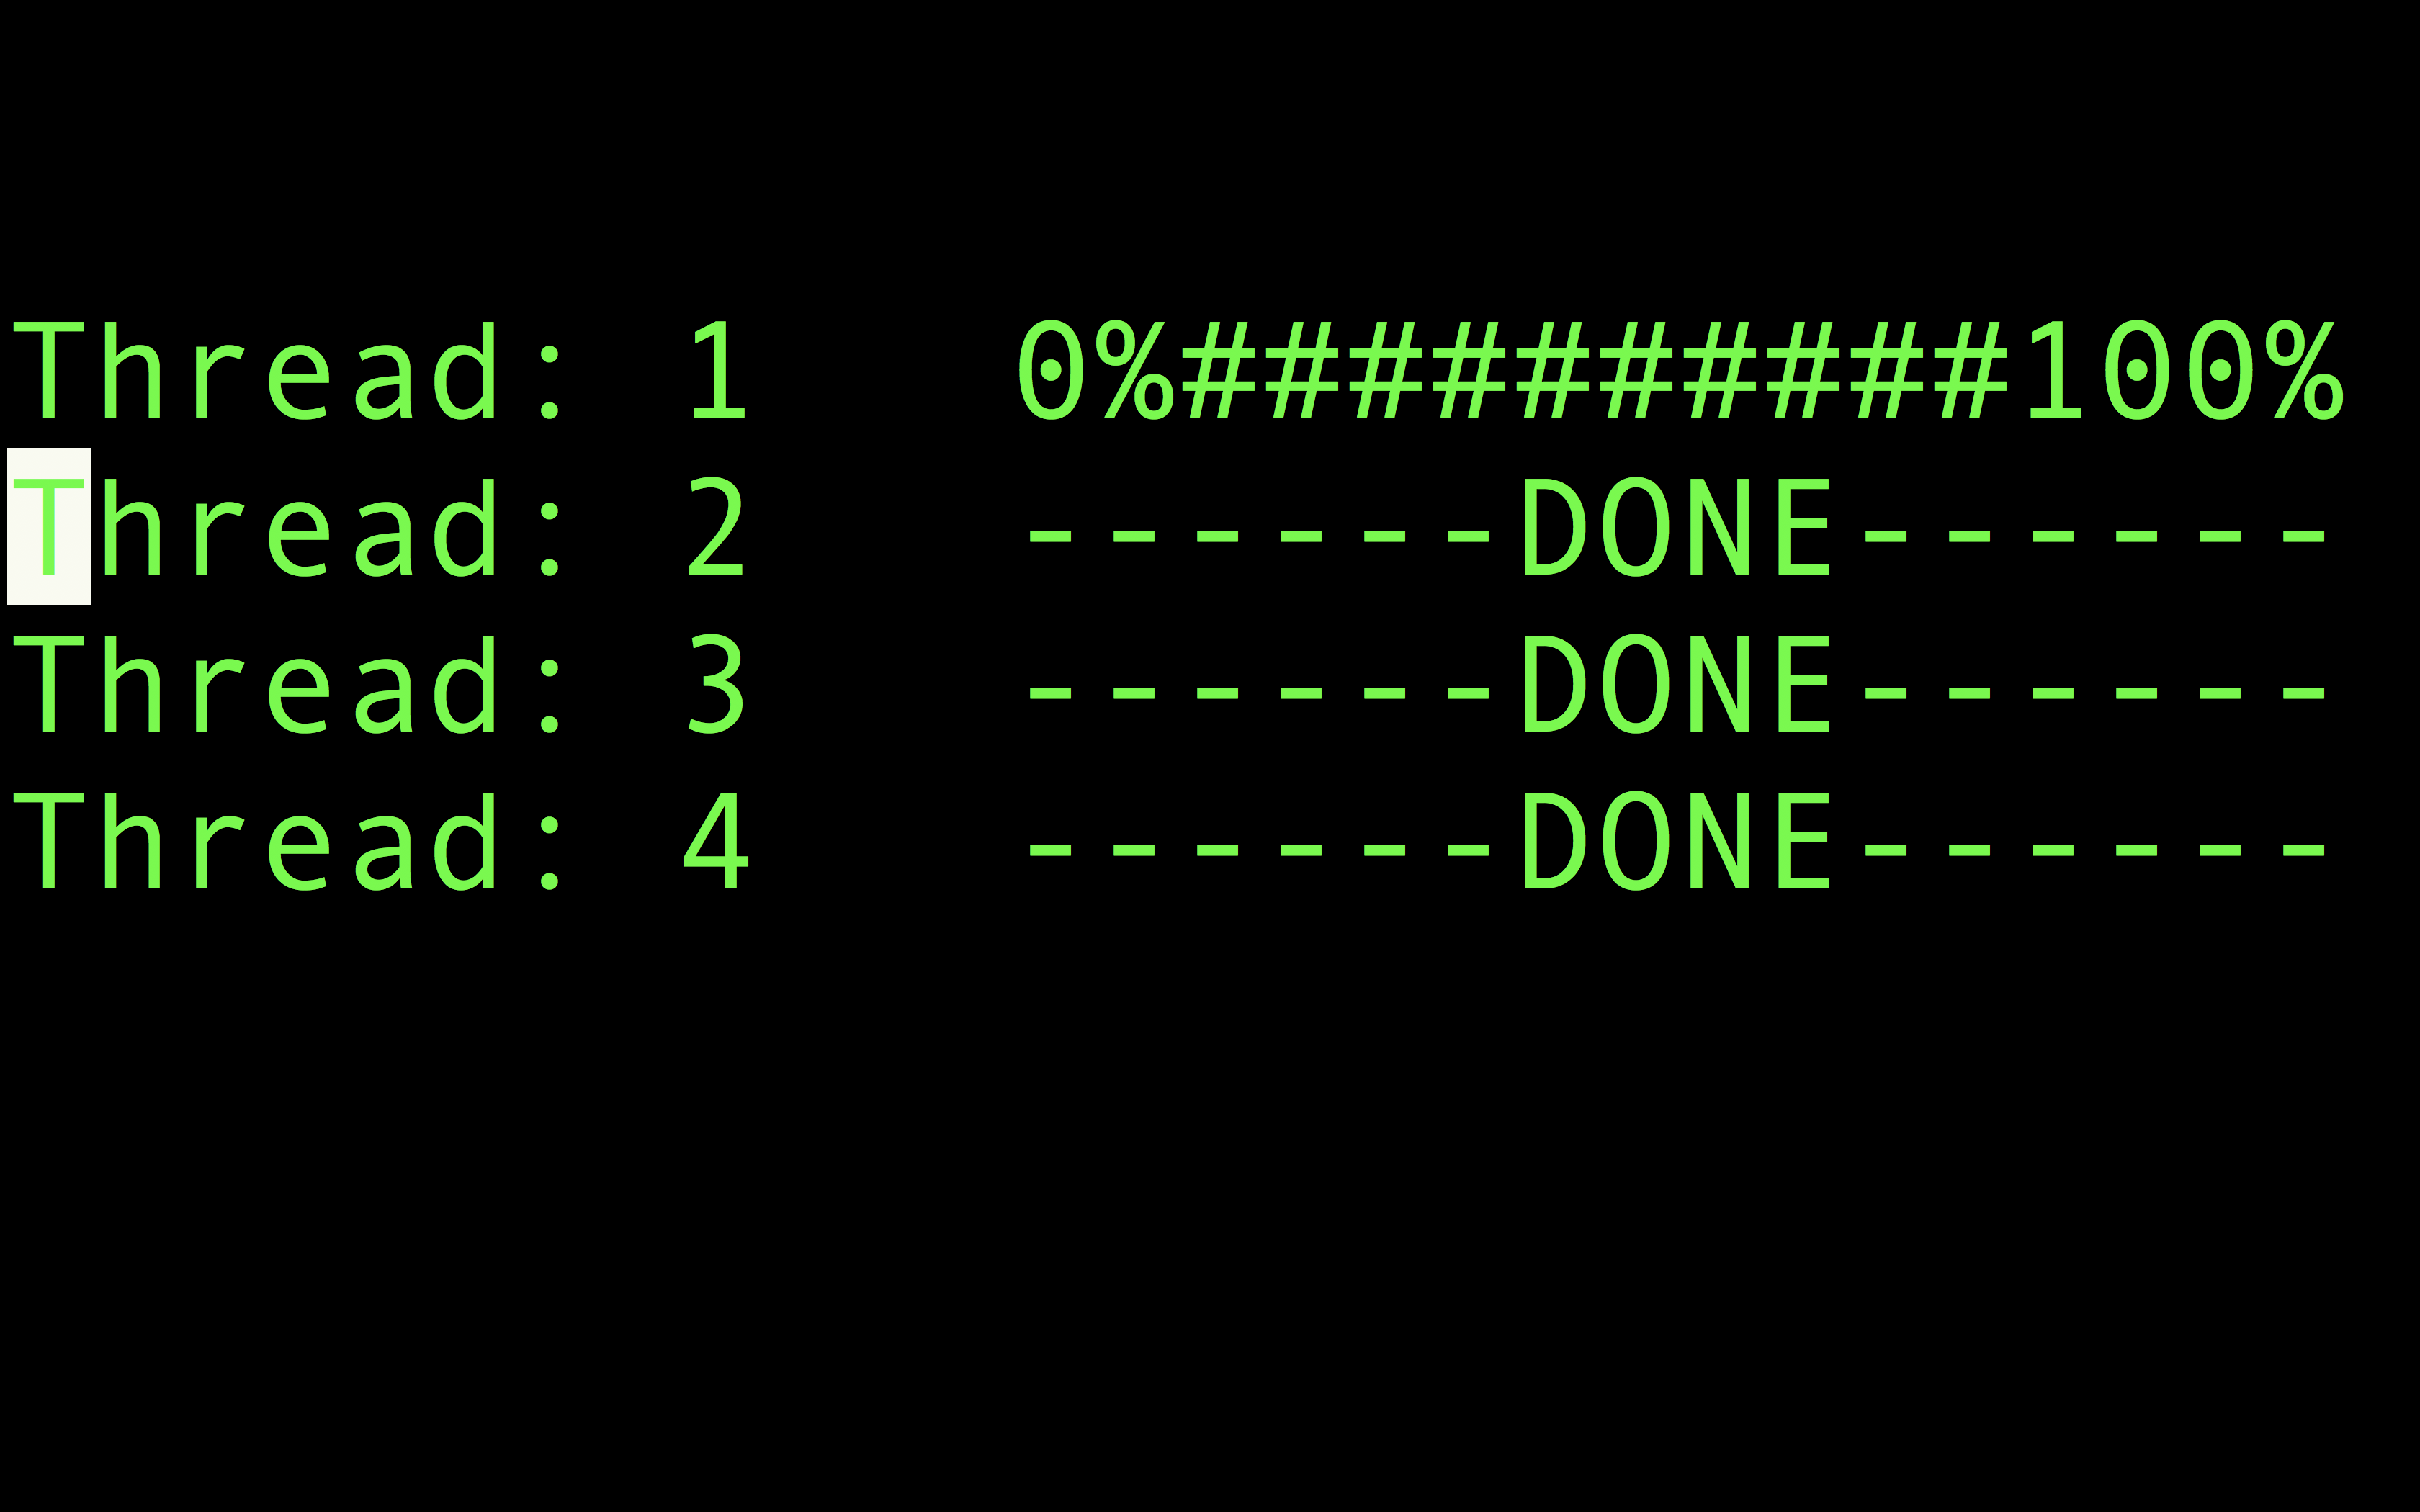
\includegraphics[width=1.11\linewidth]{method/bilder/5}
    \end{subfigure}
    \caption{A progress bar was made for the program. It shows the progress for each individual thread. The progress bar works for 1 to 4 threads. More then 4 threads might look funny. By the way, we are A students in the newly announced PRO101 subject. }
    \label{fig:progress}
\end{figure}
\footnotemark
\footnotetext{
    \href
    {https://shortridgedailyecho.org/wp-content/uploads/2017/08/definition-procrastination.png}
    {
    \color{blue}{PRO101: Procrastination for students}
    }
    }
% \animategraphics{12}{gif-}{1}{32}